\section{Aufgenommene Datenmenge}
\label{sec:DymelData}
\texttt{DymelData} ist eine Datenmenge, die mit dem \texttt{Recorder} (siehe Sektion \ref{sec:recorder}) erstellt wurde. Sie umfasst insgesamt 14410 Gesten in unterschiedlichen Konfigurationen. Sie wurde
einerseits aufgenommen, um unter den vorort bestehenden Lichtverhältnissen die Modelle miteinander vergleichen zu können und andererseits, um Test- und Trainingsdaten für Nullgesten bereitzustellen. In den
bisherigen Datenmengen enthält nur ein geringer Anteil Nullgesten.
\newline
\newline
\subfigbox{
\subfigure[Geringe Helligkeit]{\label{subfig:light_low}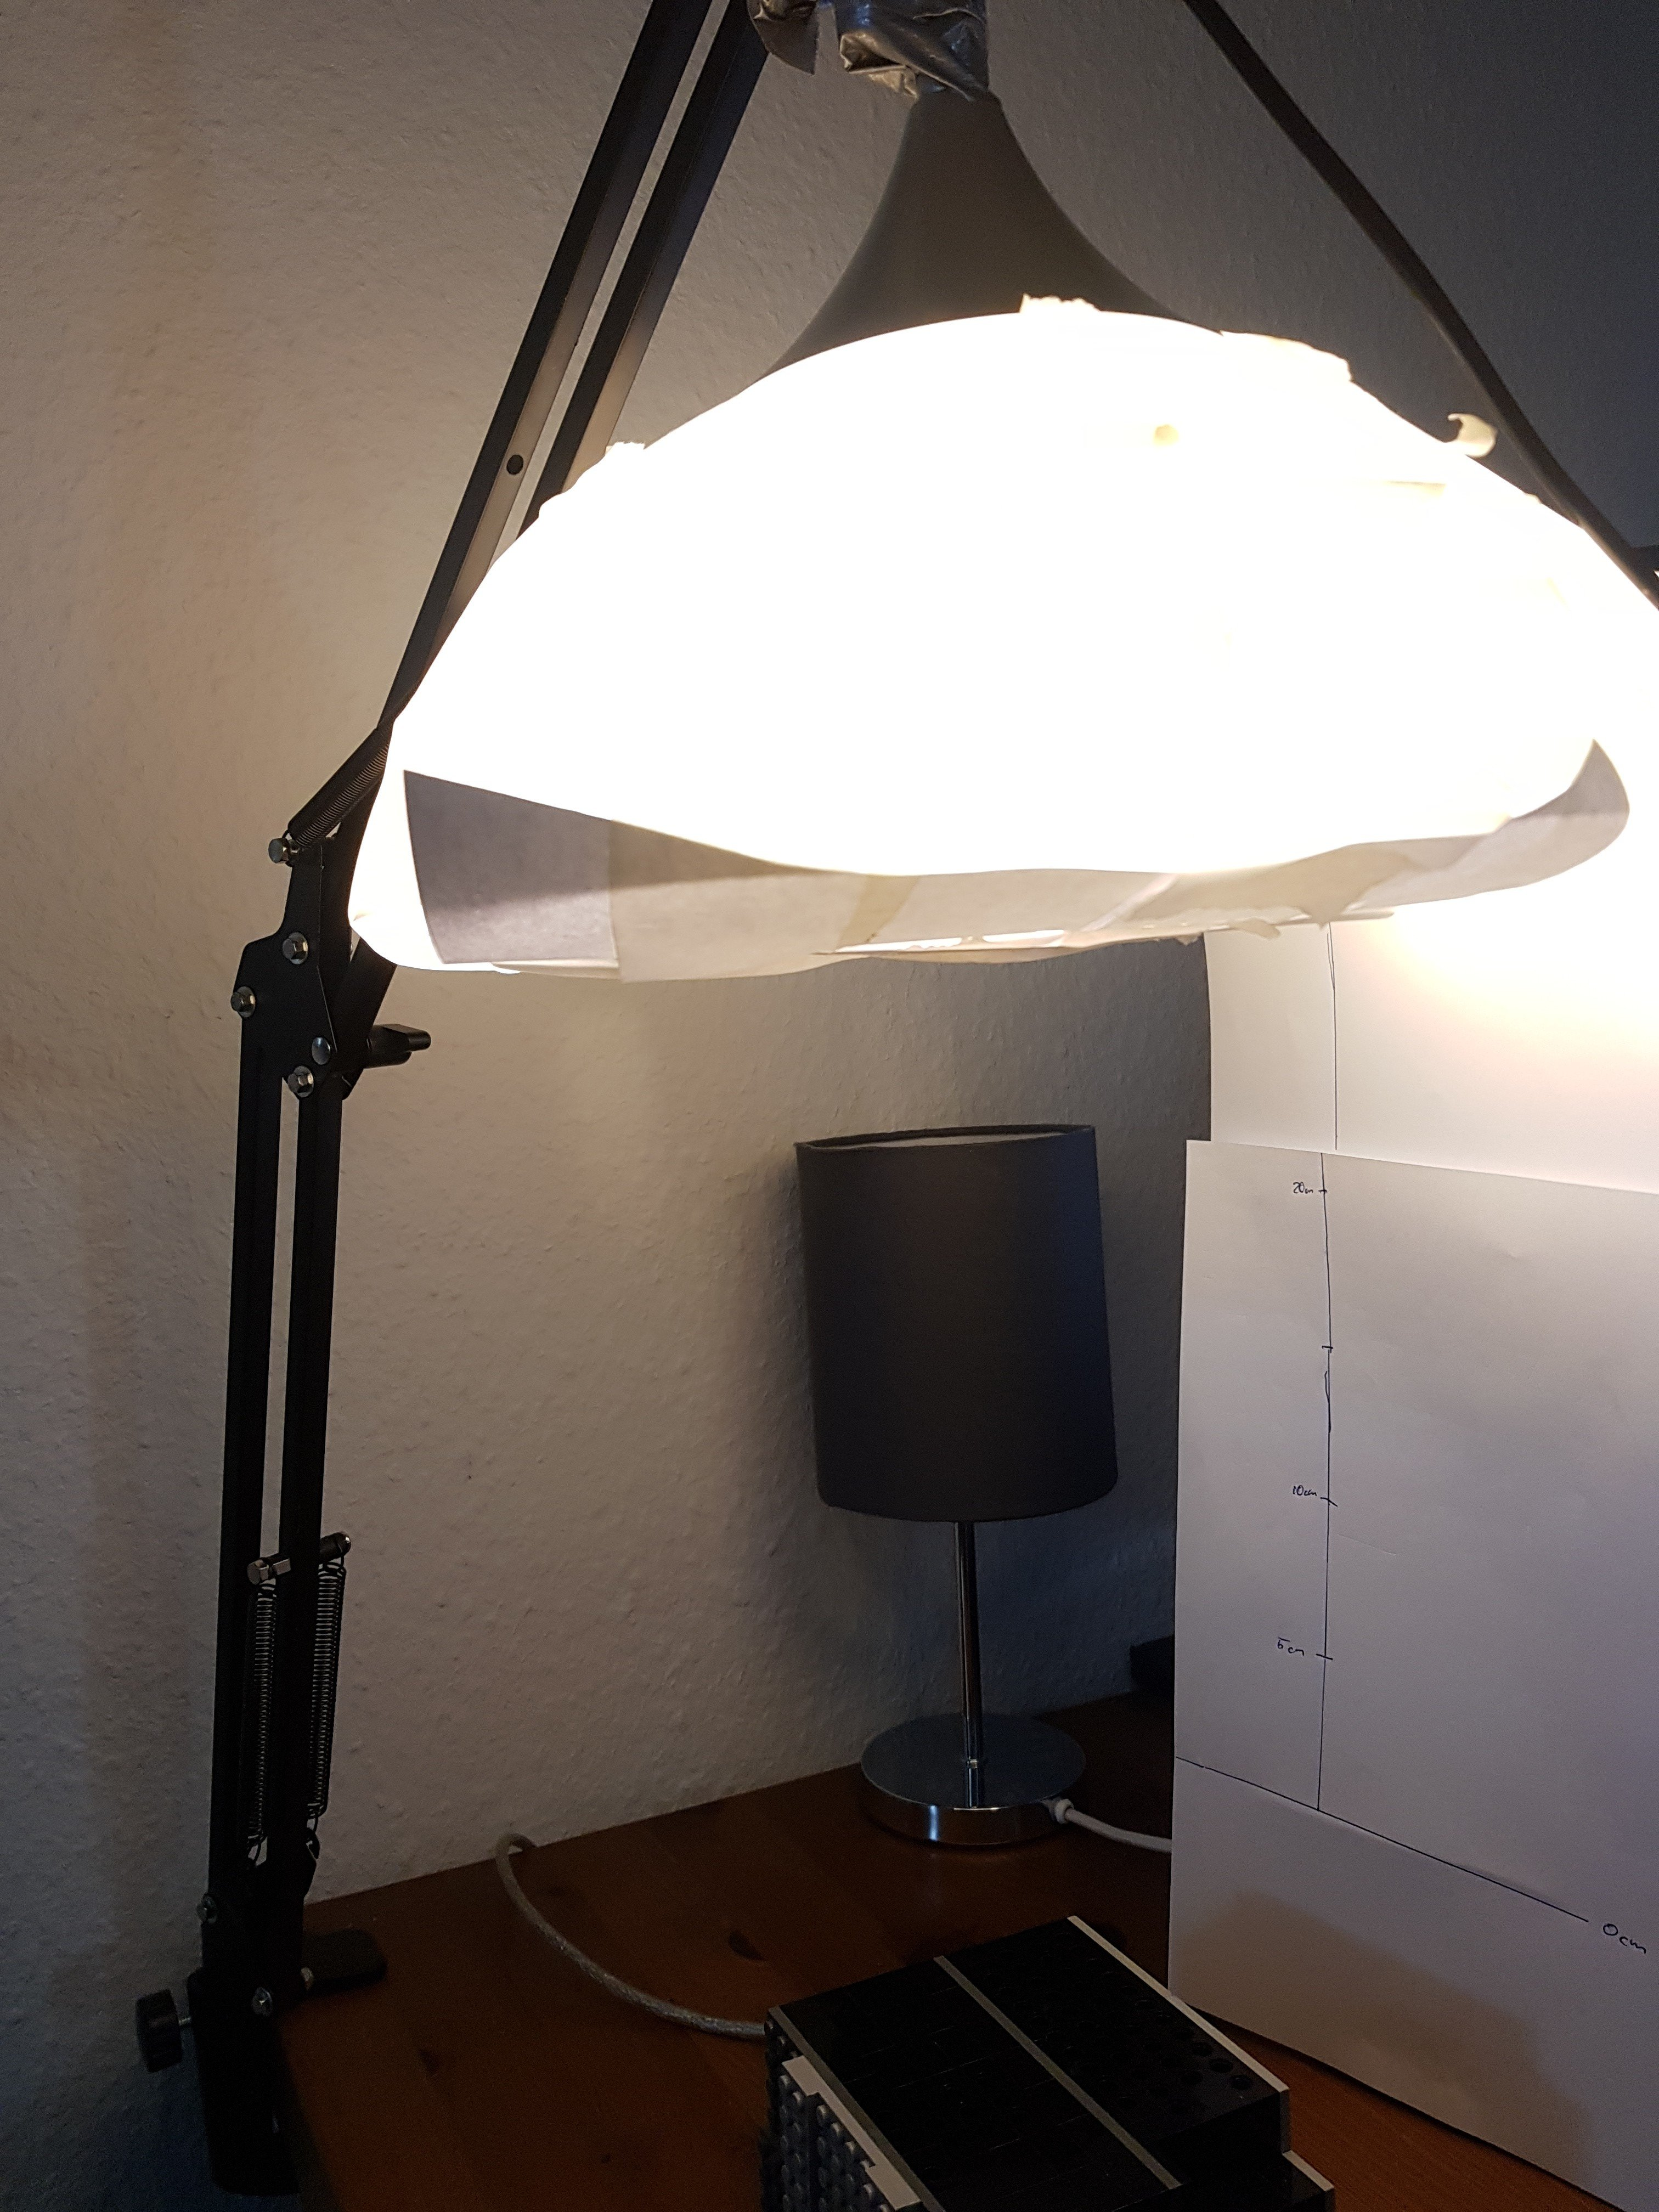
\includegraphics[width=0.33\linewidth]{images/light_low.jpeg}}\hfill%
\subfigure[Halbe Helligkeit]{\label{subfig:light_medium}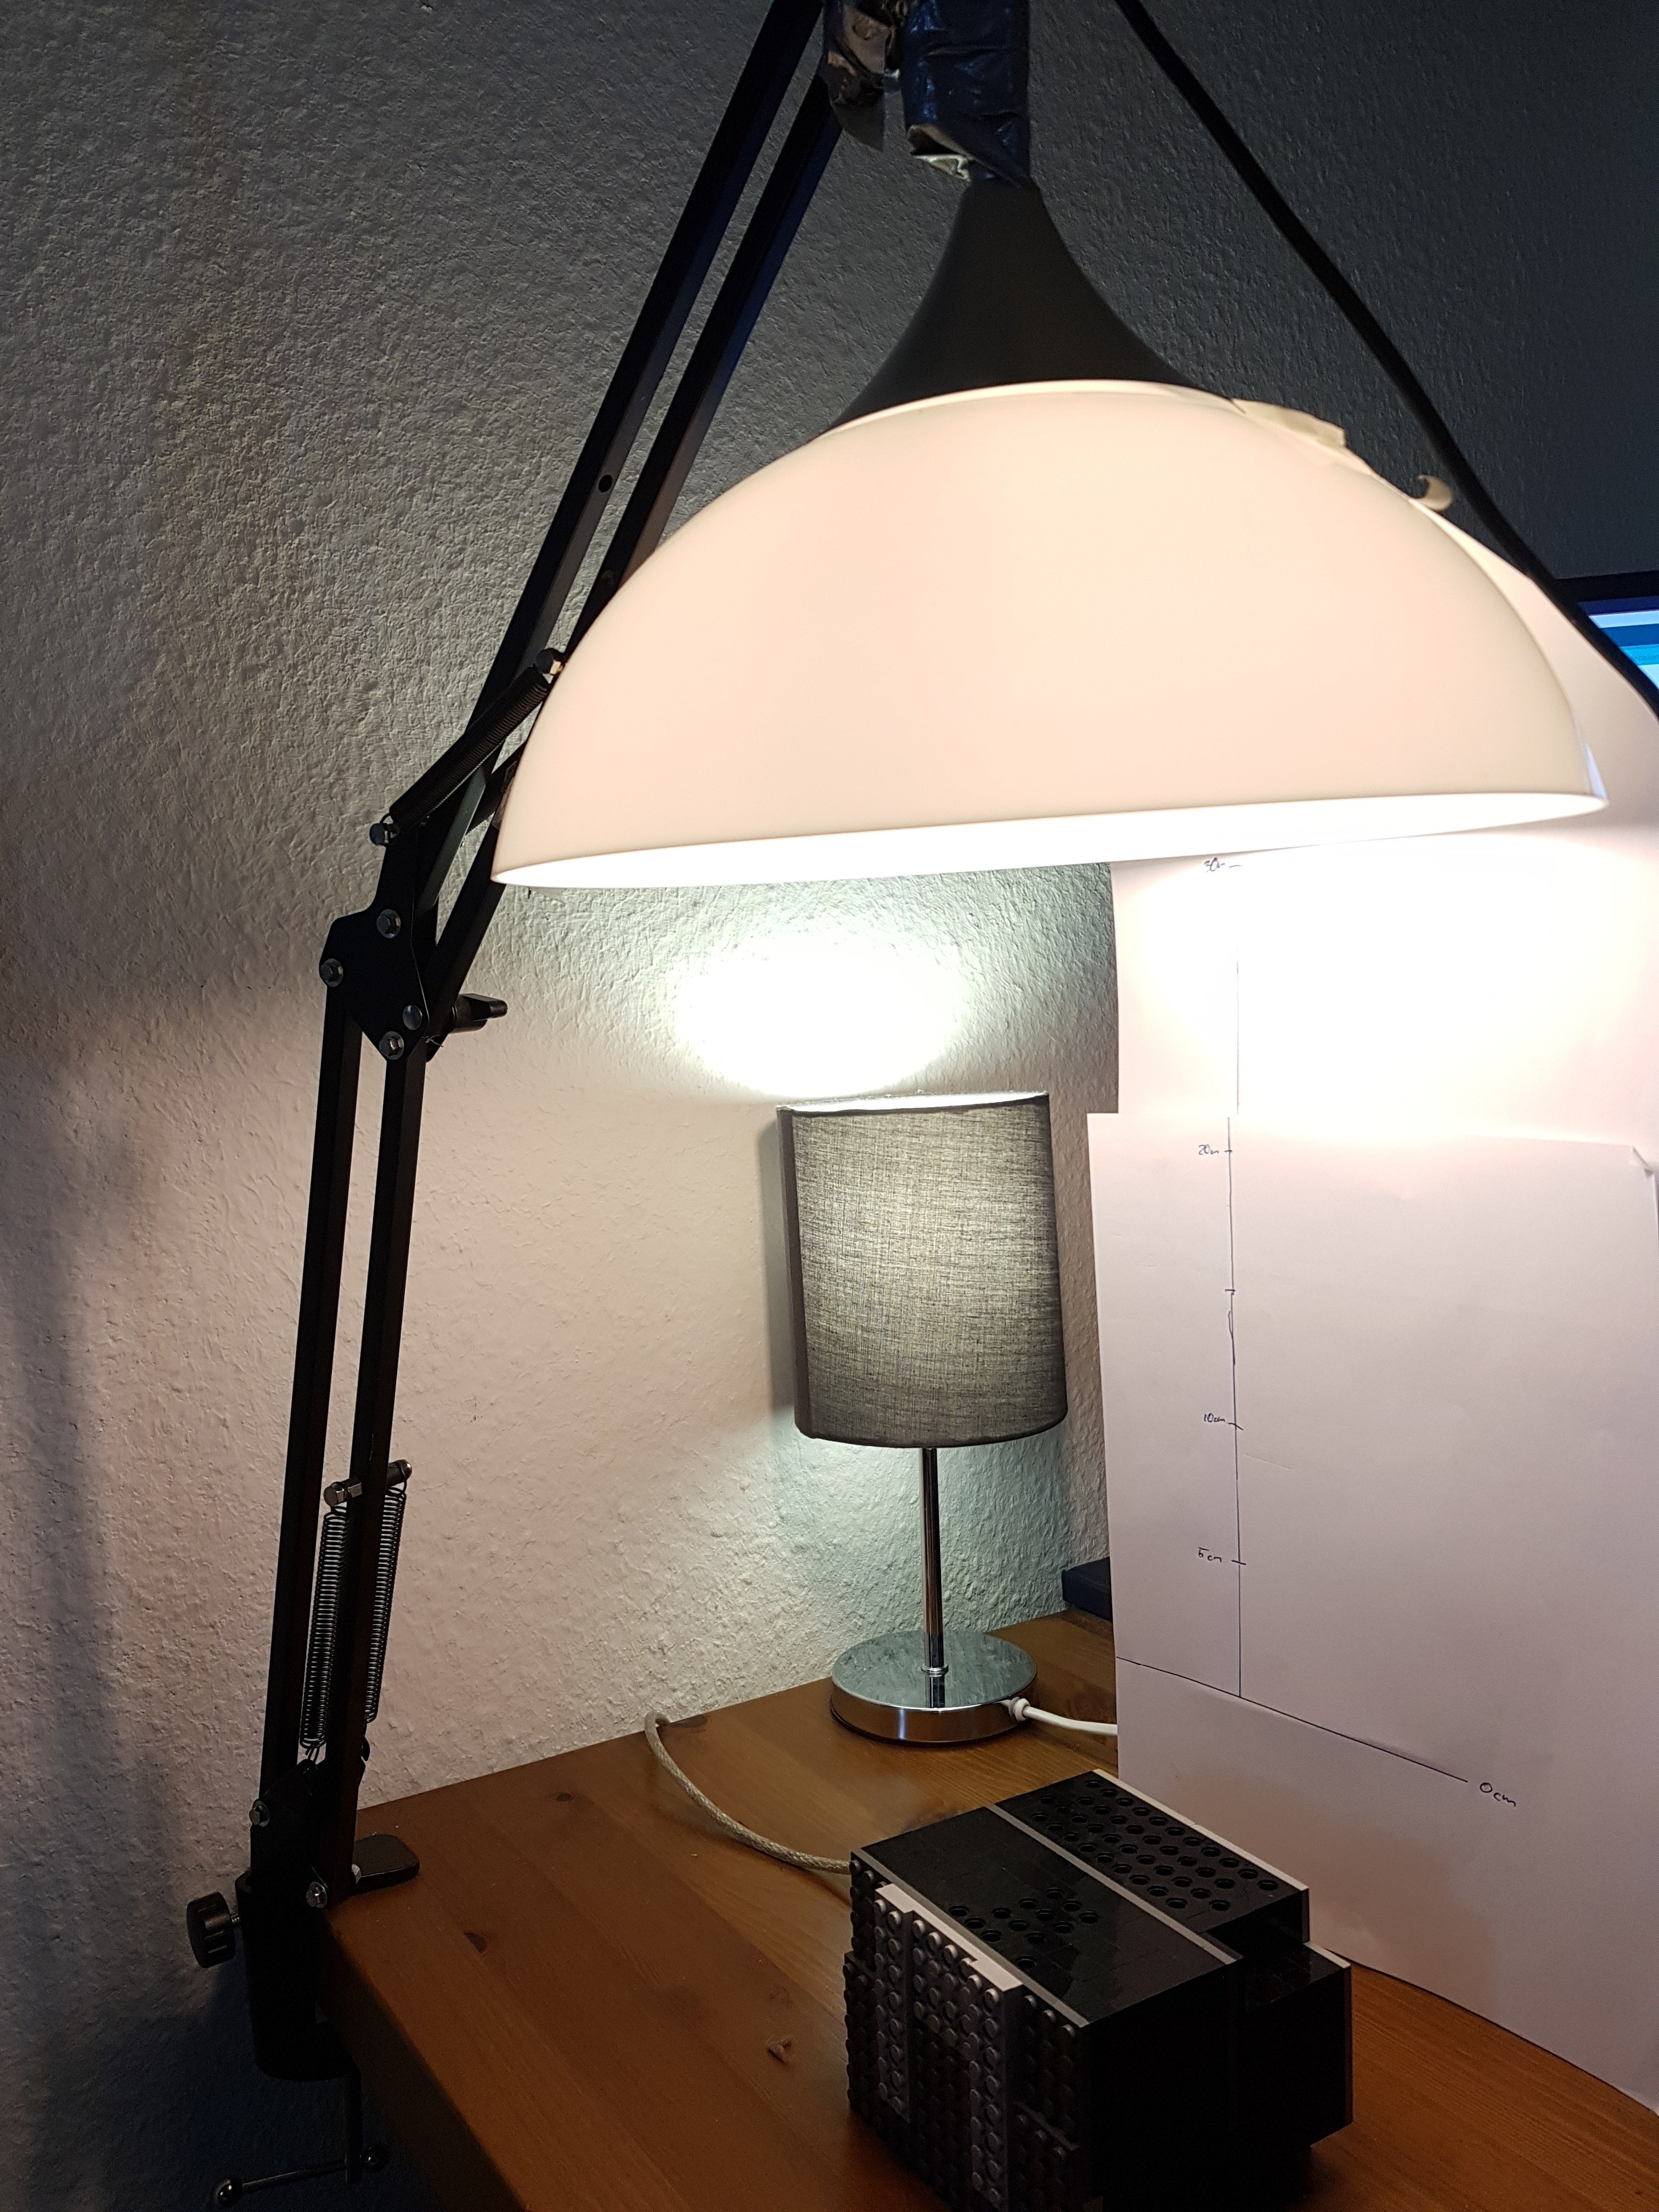
\includegraphics[width=0.33\linewidth]{images/light_medium.jpeg}}\hfill%
\subfigure[Hohe Helligkeit]{\label{subfig:light_high}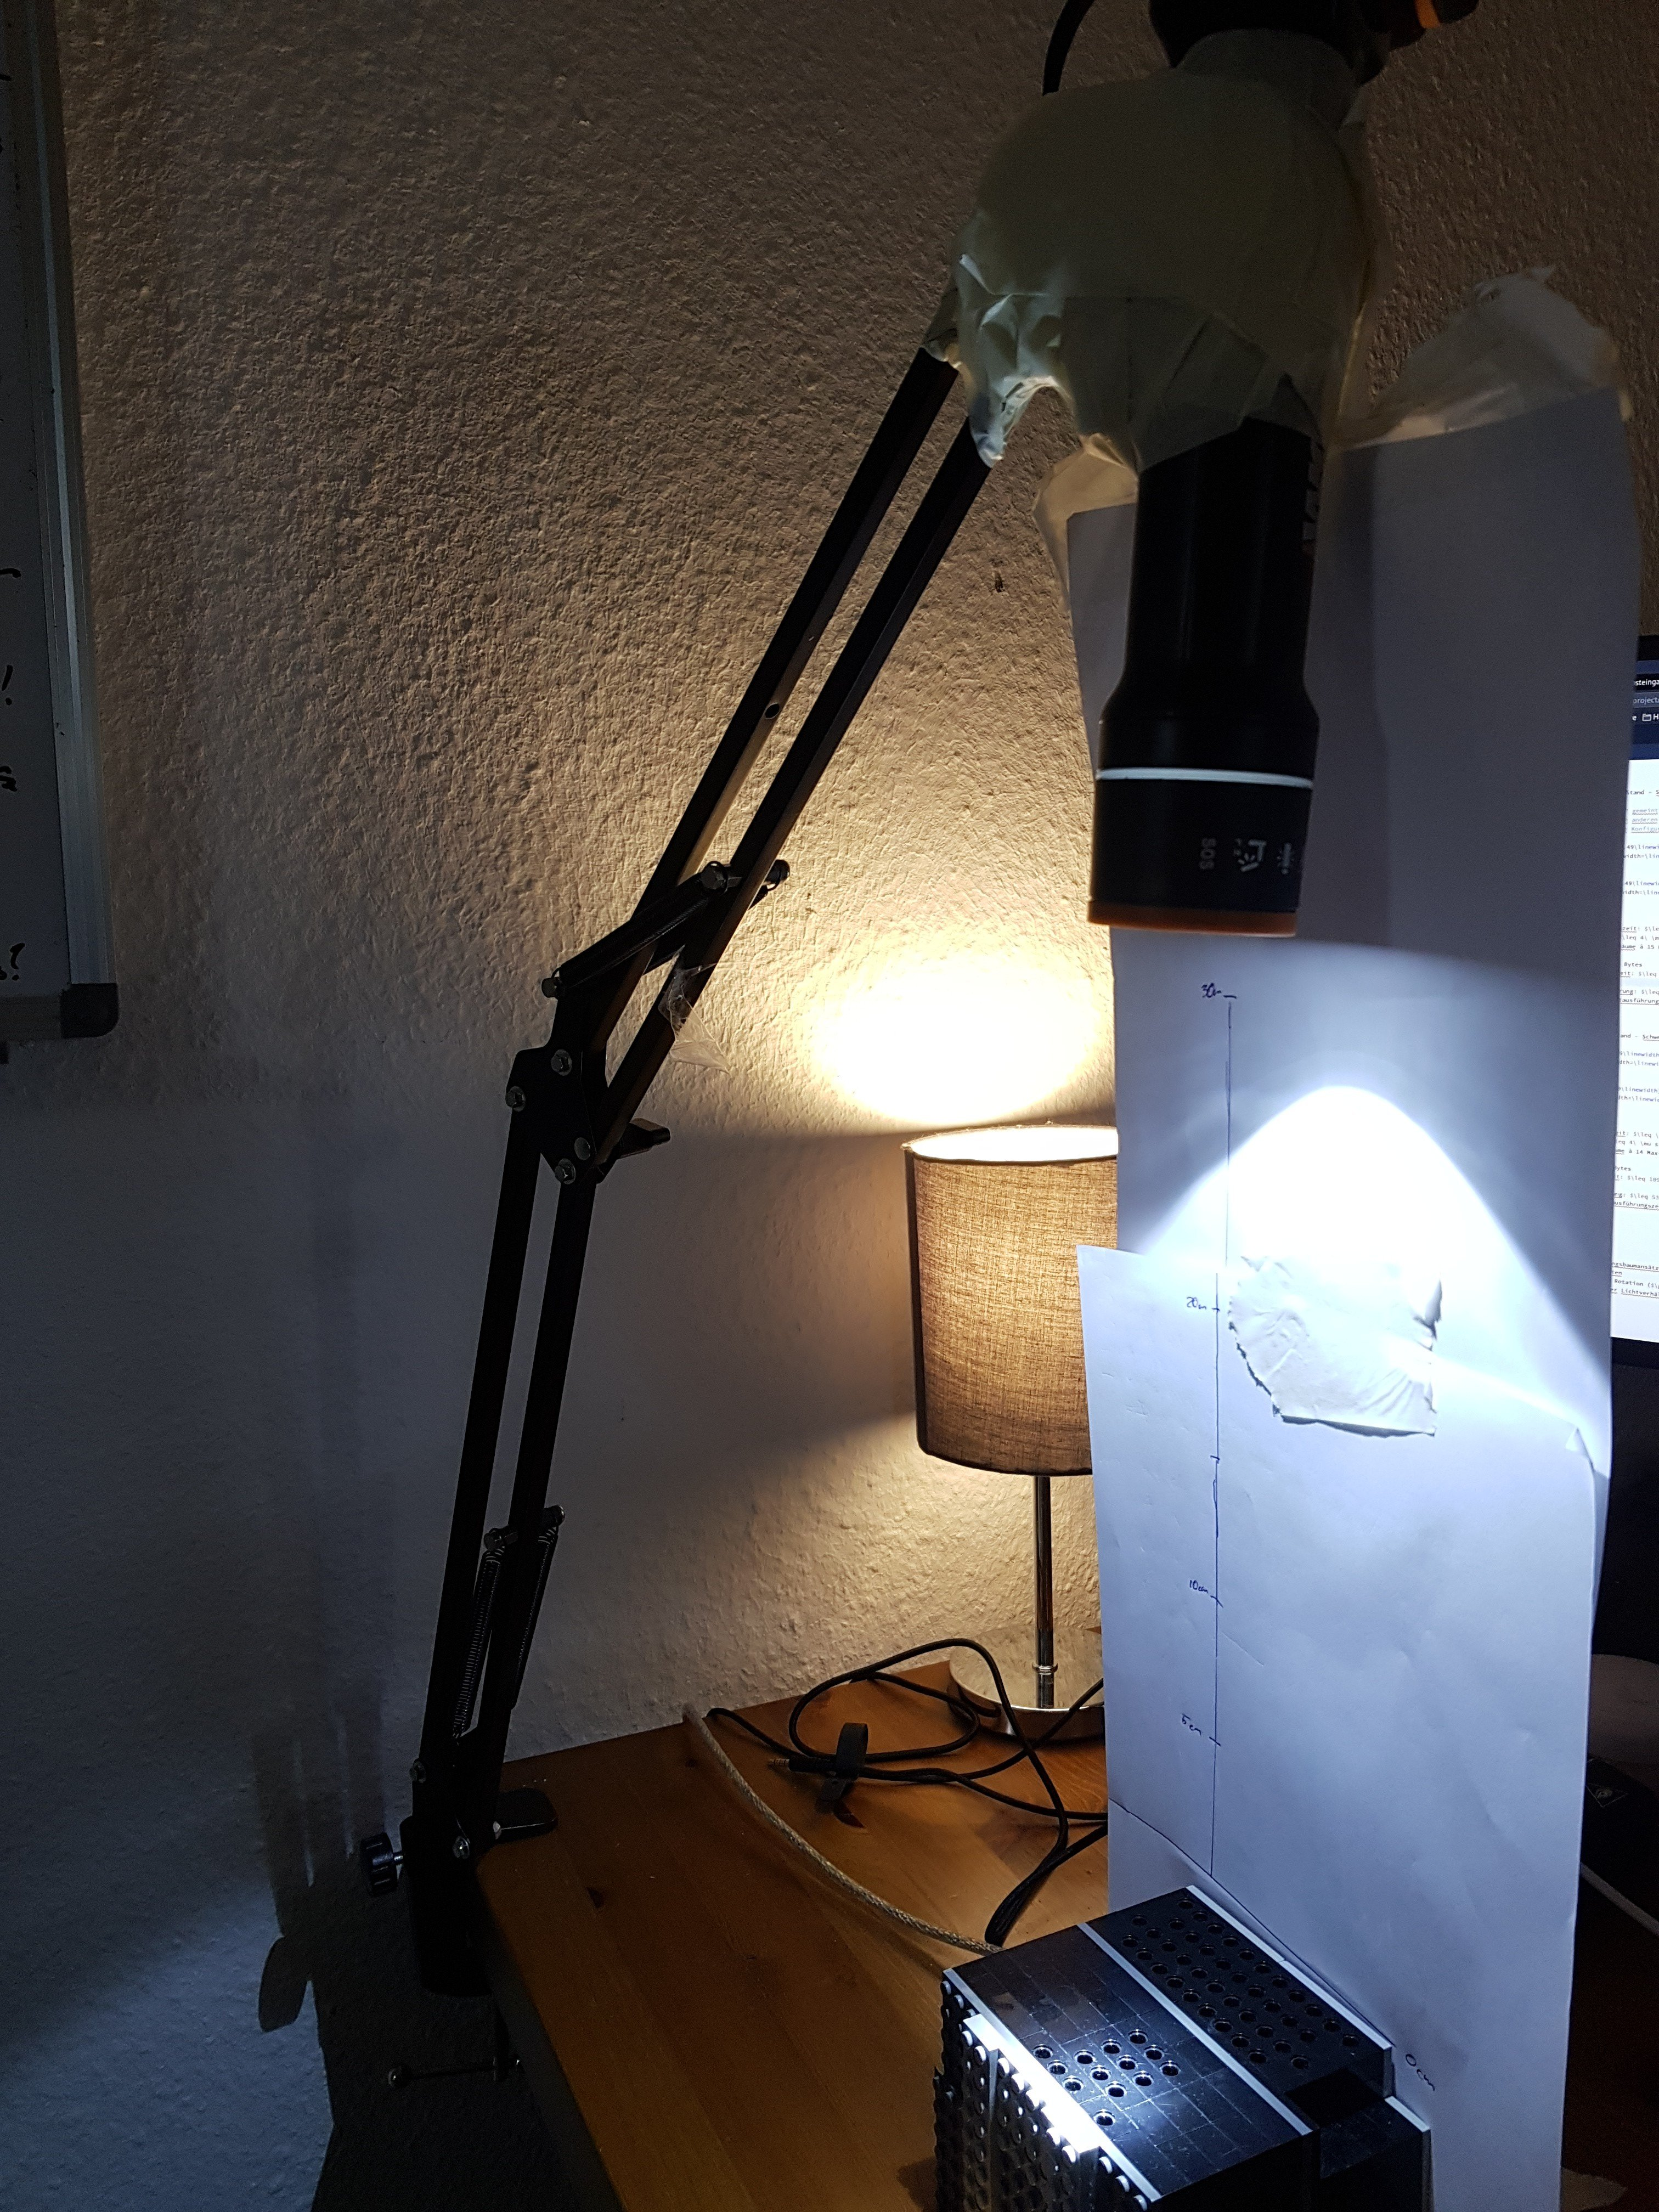
\includegraphics[width=0.33\linewidth]{images/light_high.jpeg}}%
}{Verschiedene Helligkeitsstufen unter denen die Gesten von \texttt{DymelData} aufgenommen wurden.}{fig:different_lights}
Jede Handgeste wurde unter jeder Konfiguration ca. 100 mal aufgenommen bei 90 Bildern pro Sekunde. Insgesamt wurden in 3 Lichtverhältnisse und 4 Distanzen, 6 verschiedene Gesten (Links nach Rechts,
Rechts nach Links, Oben nach Unten, Unten nach Oben und 2 NullGesten) jeweils schnell und langsam aufgenommen. Die Gesten wurden in den Abständen 5 cm, 10 cm, 20 cm und 25 cm aufgenommen.
\newline
\newline
Die \glqq Geringe\grqq\ Helligkeit war im Durchschnitt bei ca. 140, \glqq Halbe\grqq\ Helligkeit bei ca. 659, \glqq Hohe\grqq\ Helligkeit bei ca. 908. Alle Helligkeiten haben das 3x3-Array
relativ gleichmäßig ausgeleuchtet. Bei den Lichtquellen \ref{subfig:light_low} und \ref{subfig:light_medium} wurde eine Schirmlampe verwendendet. Dadurch wurde das Licht relativ breit gestreut,
wodurch der Kontrast mit vergrößender Distanz abgenommen hat. Bei \ref{subfig:light_high} wurde eine Punktlichtquelle verwendet, wodurch der Kontrast über alle Distanzen sehr stark ist.
\newline
\newline
Insgesamt wurden 2 Typen von Nullgesten aufgenommen. Die erste Nullgeste geht \textit{Oben} rein, verschieden weit in Richtung \textit{Unten} und kehrt anschließend um, um bei \textit{Oben} wieder rauszukommen.
Die zweite Nullgeste geht \textit{Oben} rein, verschieden weit in Richtung \textit{Unten} und anschließend \textit{Rechts} wieder raus.
\newline
\newline
Die resultierenden Handgesten werden anschließend um 90°, 180° und 270° rotiert, um die equivalenten Nullgesten aus den anderen Richtungen zu inferieren. Insgesamt enstehen dadurch 19400 Nullgesten.
\newline
\newline
Um zu testen wie gut das Model sich gegenüber verschiedene Lichtverhältnisse generalisiert hat, ist es nötig mehr als nur 3 Helligkeitsstufen zu testen. Aus diesem Grund wurde aus der Gestenmenge mit
der Helligkeit \glqq Gering\grqq\ eine synthetische Testmenge generiert.
\newline
\newline
Dabei wurden jeweils 20 Duplikate der Datenmenge erstellt mit einem Helligkeitsoffset zwischen 50 und 1000 und einer Skalierung zwischen 0,5 und 10. Diese Datenmengen wurden zu einer Testmenge zusammengefügt.